\paragraph*{Single-Task Imitation Learning}\mbox{}\\
This paragraph will review the research conducted in the context of \textit{ Single-Task Imitation Learning}. Specifically, within the scope of robotic manipulation problems, the term ``Single-Task" indicates that the learned policy $\pi^{L}$ can perform only the specific task it has been trained on. For example, if the task involves a pick-and-place operation with a fixed place position, the model cannot handle variations in the place location. Additionally, the focus will be primarily on methods that use high-dimentional state representations, such as images, processed by deep architectures to solve the problem.

In this scenario, the scientific literature extends far back in time. One of the seminal works in this field was proposed in 1988 by Pomerleau, who introduced \textit{ALVINN} \cite{pomerleau1988alvinn}. ALVINN is an autonomous vehicle driving system based on a Neural Network that predicts the steering angle from a synthetic camera image input. The network was trained on pairs of (image, steering angle), with the training procedure framed as a supervised classification problem. This was achieved by discretizing the steering angle into 45 units. Pomerleau's work immediately highlighted the issue of \textbf{compounding error}, which arises from the \textbf{covariate shift phenomenon}. This issue occurs because an action $a_{t}$ influences the subsequent state $s_{t+1}$, which becomes the next sample, thereby violating the i.i.d. assumption of Supervised Learning. This results in a test-data distribution that may differ from the training one. This phenomenon has significant consequences on the expected performance of the system and is addressed by methods discussed in the paragraph on \textit{Interactive Imitation Learning}.

Despite the covariate-shift problem, \cite{zhang2018deep_vr_teleoperation} showed that very interesting performance can be obtained in the context of Robot Manipulation, by means of Behavioral Cloning and high quality demonstrations given by teleportation system. In this work, a Convolutional Neural Network was trained to predict the desired linear-velocity, angular-velocity of the end-effector, and the binary gripper state (open/close), given in input the current RGB-D observation of the scene, and the position of three points of the end-effector, during the last 5 time-steps (Figure \ref{fig:deep_bc}). The system was tested on 10 tasks, and the performance are reported in Table \ref{table:deep_vr_teleoperation_results}. The proposed system achieved a high success rate while evaluating all the tasks. The tests were carried out from different initial conditions but still quite similar to those present in the training set (e.g., the initial object positions have been uniformly distributed within the training regime, with random local variations around these positions). The analysis of failure cases showed that the leading cause of errors was the inability to detect critical points in the task execution, such as closing/opening the gripper to pick/place the object or detect the position of the object of interest in order to avoid collision with it.
\begin{figure}[bt]
    \centering
    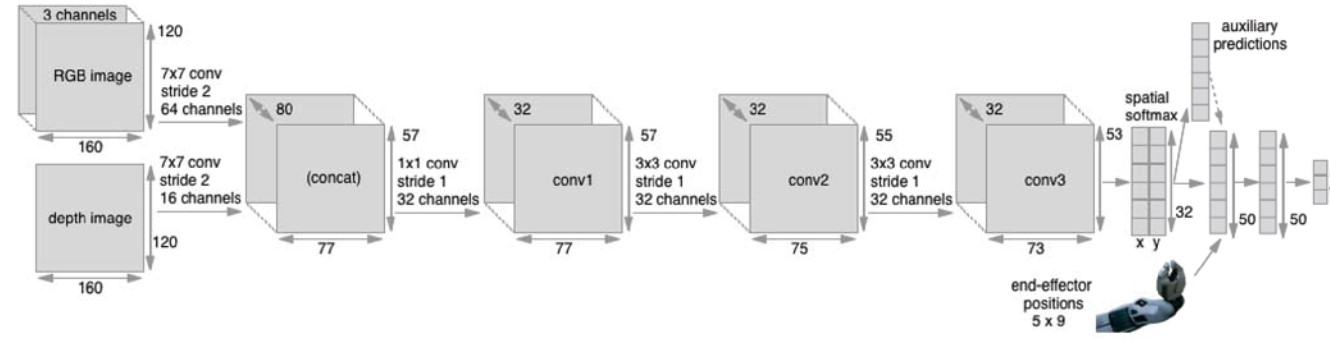
\includegraphics[width=0.9\textwidth]{figures/images/deep_imitation_bc/deep_imitation_bc.jpg}
    \caption{Architecture proposed in~\cite{zhang2018deep_vr_teleoperation}}
    \label{fig:deep_bc}
\end{figure}

% \usepackage{graphicx}
% \usepackage{hhline}


\begin{table}
    \centering
    \caption{Statistics of Training set, and Test Success rate~\cite{zhang2018deep_vr_teleoperation}}
    \label{table:deep_vr_teleoperation_results}
    \resizebox{\linewidth}{!}{%
    \begin{tabular}{|c|c|c|c|c|c|c|c|c|c|c|} 
    \hline
    \textbf{Task} & \textbf{Reaching} & \textbf{Grasping} & \textbf{Pushing} & \textbf{Plane} & \textbf{Cube} & \textbf{Nail} & \begin{tabular}[c]{@{}c@{}}\textbf{Grasp-}\\\textbf{and-}\\\textbf{Place}\end{tabular} & \begin{tabular}[c]{@{}c@{}}\textbf{Grasp-}\\\textbf{Drop-}\\\textbf{Push}\end{tabular} & \begin{tabular}[c]{@{}c@{}}\textbf{Grasp-}\\\textbf{Place-x2}\end{tabular} & \textbf{Cloth} \\ 
    \hhline{|===========|}
    \#demo & 200 & 180 & 175 & 319 & 206 & 215 & 109 & 100 & 60 & 100 \\ 
    \hline
    \begin{tabular}[c]{@{}c@{}}demo duration \\(min)\end{tabular} & 13.7 & 11.1 & 16.9 & 25.0 & 12.7 & 13.6 & 12.3 & 14.5 & 11.6 & 10.1 \\ 
    \hline
    \begin{tabular}[c]{@{}c@{}}Test success rate\\(\%)\end{tabular} & 91.6 & 97.2 & 98.9 & 87.5 & 85.7 & 87.5 & 96.0 & 83.3 & 80.0 & 97.4 \\
    \hline
    \end{tabular}
    }
    \end{table}
Generally speaking, when working with these types of systems, there are various aspects and design choices to consider. These include the selection of the architecture (e.g., temporal-dependent or independent), the type of demonstration (human-generated or machine-generated), the quantity of demonstrations, and so on. The authors in \cite{mandlekar2022matters} identify a set of challenges in \textit{Learning from Offline Human Demonstrations} context and propose an extensive study, offering valuable insights for future work.

Specifically, the authors tested three Imitation Learning algorithms and two Offline Reinforcement Learning algorithms in both simulated and real-world manipulation tasks (Figure \ref{fig:what_matters_task}). The study primarily focused on analyzing the following aspects:

\begin{enumerate}
    \item \textit{Source of Demonstrations}: Comparing system performance with demonstrations generated by hand-written policies (MG), proficient human demonstrators (PH), and multiple human demonstrators with varying levels of expertise in teleoperation (MH).
    \item \textit{Observation Space}: Comparing the performance of methods based on the type of input, whether low-dimensional (gripper pose, gripper fingers position, object position) or image-based (visual observation, gripper pose, gripper fingers position).
\end{enumerate}
\begin{figure}[t]
    \centering
    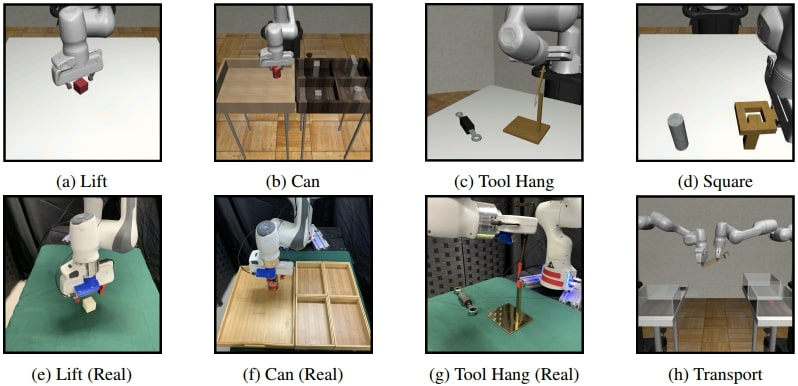
\includegraphics[width=0.9\textwidth]{figures/images/what_matters/task.jpg}
    \caption{The set of tasks presented in the benchmark \cite{mandlekar2022matters}.}
    \label{fig:what_matters_task}
\end{figure}

Specifically, by extrapolating the most important results from this study (Table \ref{table:what_matters_res_low_dimensional}), it can be observed that the most promising architecture is the recurrent BC-RNN, particularly for datasets composed of multi-human demonstrations (MH). This architecture outperforms even state-of-the-art offline reinforcement learning algorithms, which tend to struggle with datasets containing trajectories of varying quality.

In conclusion, for real-world tasks, the BC-RNN architecture achieved a success rate of \textbf{96.7}\% on the lift task, \textbf{73.3}\% on the can task, and \textbf{3.3}\% on the tool-hang task. These results are noteworthy, as they essentially demonstrate the feasibility of training a proficient system from offline human demonstrations. However, several aspects must be considered, such as the simplicity of the test scenarios, which include only one object without any distractors, and the potential benefit of incorporating contact information for contact-rich manipulation tasks like the tool-hang.

% \usepackage{graphicx}
% \usepackage{hhline}


\begin{table}
    \centering
    \caption{Results are presented on tasks performed in a high-dimensional observation space for simulated environments. PH refers to \textit{Proficient Human}, which represents trajectories collected by a single expert human demonstrator with extensive experience in teleoperating the robot. MH refers to \textit{Multi Human}, which represents trajectories collected by multiple human operators with varying levels of expertise in teleoperation.}
    \label{table:what_matters_res_low_dimensional}
    \resizebox{\linewidth}{!}{%
    \begin{tabular}{|c|c|c|c|c|} 
    \hline
    \textbf{Dataset} & \textbf{BC} & \textbf{BC-RNN} & \textbf{BCQ} & \textbf{CQL} \\ 
    \hhline{|=====|}
    Lift $(\mathrm{PH})$ & $\mathbf{1 0 0 . 0} \pm \mathbf{0 . 0}$ & $\mathbf{1 0 0 . 0} \pm \mathbf{0 . 0}$ & $\mathbf{9 8 . 0} \pm \mathbf{1 . 6}$ & $52.0 \pm 13.0$ \\ 
    \hline
    Can $(\mathrm{PH})$ & $\mathbf{9 7 . 3} \pm \mathbf{1 . 9}$ & $\mathbf{9 8 . 0} \pm \mathbf{0 . 9}$ & $86.7 \pm 2.5$ & $0.7 \pm 0.9$ \\ 
    \hline
    Square $(\mathrm{PH})$ & $62.0 \pm 4.9$ & $\mathbf{8 2 . 0} \pm \mathbf{0 . 0}$ & $41.3 \pm 4.1$ & - \\ 
    \hline
    Transport $(\mathrm{PH})$ & $55.3 \pm 6.2$ & $\mathbf{7 2 . 0} \pm \mathbf{4 . 3}$ & $0.7 \pm 0.9$ & - \\ 
    \hline
    Tool Hang $(\mathrm{PH})$ & $20.0 \pm 5.9$ & $\mathbf{6 7 . 3} \pm \mathbf{4 . 1}$ & $3.3 \pm 0.9$ & - \\ 
    \hhline{|=====|}
    Lift $(\mathrm{MH})$ & $\mathbf{1 0 0 . 0} \pm \mathbf{0 . 0}$ & $\mathbf{1 0 0 . 0} \pm \mathbf{0 . 0}$ & $93.3 \pm 0.9$ & $11.3 \pm 9.3$ \\ 
    \hline
    Can $(\mathrm{MH})$ & $85.3 \pm 0.9$ & $\mathbf{9 6 . 0} \pm \mathbf{1 . 6}$ & $77.3 \pm 6.8$ & $0.0 \pm 0.0$ \\ 
    \hline
    Square $(\mathrm{MH})$ & $46.0 \pm 1.6$ & $\mathbf{7 6 . 7} \pm \mathbf{3 . 4}$ & $17.3 \pm 7.5$ & - \\ 
    \hline
    Transport $(\mathrm{MH})$ & $18.7 \pm 2.5$ & $\mathbf{4 2 . 0} \pm \mathbf{1 . 6}$ & $0.0 \pm 0.0$ & - \\
    \hline
    \end{tabular}
    }
    \end{table}
After this work, further research in the field of Single Task Imitation Learning, focused on exploring novel architecture \cite{shafiullah2022behavior} and learning paradigm \cite{nair2022r3m,cheng2023diffusion,shi2023waypoint}. 

Regarding the learning paradigm, the contribution presented in \cite{nair2022r3m} is particularly noteworthy. The authors introduced \textit{R3M} (Reusable Representations for Robotic Manipulation), exploring the potential of leveraging pre-trained visual backbones in the context of robotic manipulation. In traditional computer vision tasks, such as object detection, it is standard practice to use backbones pre-trained on large, general datasets and fine-tune them for specific problems, significantly reducing training time. However, this approach is not as widely adopted in robotic manipulation, mainly due to the vastly different evaluation scenarios, including variations in tasks, robot embodiments, and environments. This raises the question of whether the fine-tuning approach is also applicable to robotic manipulation problems.

To address this question, the authors in \cite{nair2022r3m} started with the Ego4D dataset \cite{grauman2022ego4d}, which contains over 3,500 hours of video footage of people engaging in a wide range of tasks, from cooking to socializing to assembling objects, across more than 70 locations worldwide. They trained a ResNet50 \cite{resnet} to generate a robust representation that could be leveraged in robotic manipulation tasks. The authors proposed a self-supervised learning procedure designed to capture the following aspects:

\begin{itemize}
    \item \textit{Temporal Dynamics}: The learned representation should account for features related to physical interactions. To achieve this, the authors introduced a \textbf{Time Contrastive Loss}, implemented as an InfoNCE loss, which creates similar embeddings for time-adjacent frames while keeping frames that are far apart in time or from different videos distinct.
    \item \textit{Semantic Meaning}: The learned representation should encode information related to the task itself. To capture this, the authors introduced a language prediction module. Given the representation for the first frames of a task $k$ ($\phi^{k}_{0}$), the representation for the $i^{th}$ frame of the same or a different task ($\phi^{j}_{i}$), and a language description $l$ referring to task $k$, the system must output a score indicating whether the transition from $\phi^{k}_{0}$ to $\phi^{j}_{i}$ corresponds to the description $l$. In this way, the system is trained to encode a representation that contains semantic features related to the task itself, enabling it to determine whether a given representation corresponds to a specific task.
\end{itemize}

In testing, the authors demonstrated that using the pre-trained R3M representation improves the overall success rate while requiring fewer demonstrations. On the Meta-World benchmark, with just 5 demonstrations, R3M achieved a success rate of nearly \textbf{$60\%$}, compared to \textbf{$30\%$} for a system trained from scratch.


Authors in \cite{cheng2023diffusion}, introduced the paradigm of ``Diffusion Learning'' in the context of policy learning for robotic manipulation. Generally speaking, the concept behind the Diffusion learning paradigm is to model the output of a network as a \textit{denoising process}. This means that,starting from $x^k$ sampled from Gaussian noise, the denoising process performs K iterations of denoising to produce a series of intermediate samples with decreasing levels of noise, $x_k, x_{k-1}, \dots, x_0$, until a desired noise-free output $x_0$ is formed. This process follows the equation in Formula \ref{eq:denoising}, where $\epsilon_{\theta}$ is the noise prediction network whose parameters are trained during learning.
\begin{equation}
    \label{eq:denoising}
    x^{k-1} = \alpha \left( x^k - \gamma \epsilon_{\theta}(x^k, k) + \mathcal{N}(0, \sigma^{2}I)\right)
\end{equation}
The authors adapted this concept to the context of robot manipulation, beginning with the observation that the denoising process can be applied to an action $a_{t}^{k}$. However, a challenge arises from the need for the model to generate an action conditioned on the current observation. This implies that the model must learn the conditional probability distribution $p(a_t \mid o_t)$ rather than the joint data distribution $p(a_t, o_t)$. To address this issue, the authors proposed the architecture illustrated in Figure \ref{fig:diffusion_model}.

\begin{figure}[t]
    \centering
    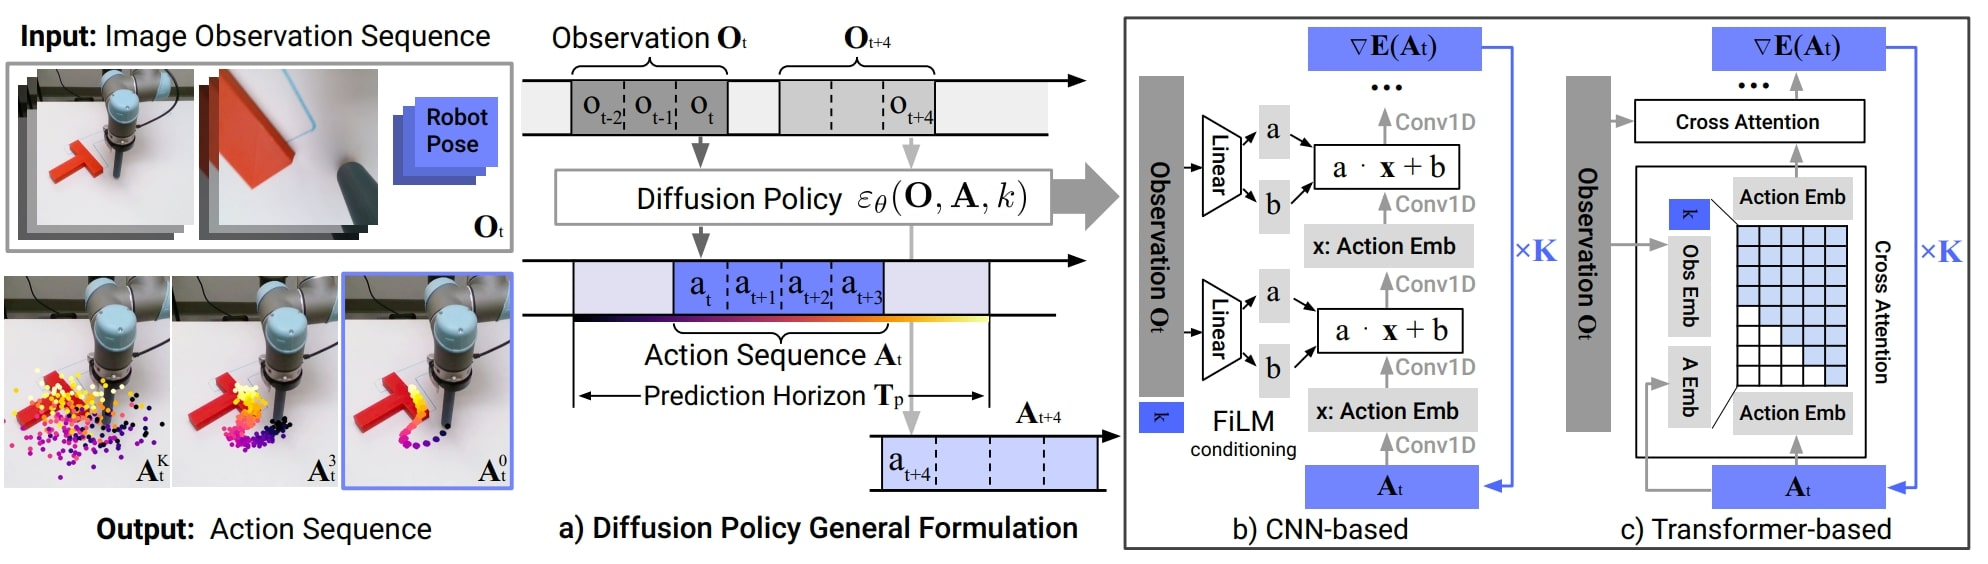
\includegraphics[width=\textwidth]{figures/images/diffusion_policy/diffusion_model.jpg}
    \caption{Architecture presented in \cite{cheng2023diffusion}. (a) General formulation, at time step $t$, the policy inputs the latest $T_o$ steps of observation data $O_t$ and outputs $T_a$ steps of actions $A_t$. (b) CNN-based Diffusion Policy, the observation feature $O_t$ is conditioned using FiLM \cite{perez2018film}. Starting with $A_t^K$ from Gaussian noise, the noise-prediction network $\epsilon_\theta$ iteratively subtracts noise to obtain the denoised action sequence $A_t^0$. (c) Transformer-based Diffusion Policy, the observation embedding $O_t$ is fed into a multi-head cross-attention layer within each decoder block, with causal attention applied to constrain each action embedding to attend only to itself and prior actions.}
    \label{fig:diffusion_model}
\end{figure}


Specifically, in both architectures, the model takes the latest $T_o$ steps of observation data $O_t$ (observation horizon) as input and predicts $T_p$ steps of actions (prediction horizon), of which $T_a$ steps of actions are executed on the robot without re-planning.

After training the system by minimizing the Mean Squared Error Loss, interesting results were obtained during testing. Specifically, the tasks depicted in Figure \ref{fig:what_matters_task} showed near-perfect results across all tasks (Lift, Can, Square, Transport, and Tool Hang), demonstrating the diffusion model's ability to better handle intrinsically noisy demonstrations from the MH set. Additionally, the Transformer-based architecture achieved an average success rate of $100\%$ on the two most complex tasks in the benchmark, Transport and Tool Hang.

Another important work related to Single-Task Imitation Learning is presented in \cite{shi2023waypoint}. The authors address the issue of compounding errors, but instead of using the Interactive Learning Paradigm (discussed in the following paragraph), they propose a novel approach. They observed that a trajectory can be decomposed into a limited number of key states or waypoints. By linearly interpolating between these waypoints, it is possible to reconstruct a demonstrated trajectory with a certain degree of accuracy, thereby mitigating the effect of compounding errors. This is because the network predicts far fewer future states compared to methods that predict every step of the trajectory. Building on this insight, the authors introduced the ``Automatic Waypoint Extraction'' (AWE) system. This system, which acts as a pre-processing tool, takes as input a trajectory $\tau$ and decomposes it into a certain number of waypoints. From these waypoints, an approximate trajectory $\hat{\tau}$ can be interpolated, with a controlled error margin.
Specifically, to decompose the original trajectory $\tau$ authors formalized the optimization problem in Formula \ref{eq:awe}, where they basically wants to find the minimum number of waypoints $W$ such that a given reconstruction loss $\mathcal{L}$ is lower than a certain margin $\eta$.
\begin{equation}
    \label{eq:awe}
    \min_{W} |W|  \ s.t. \mathcal{L}((f(W), \tau)) \le \eta
\end{equation}
They solved this problem by implementing a Dynamic Programming-based algorithm, which identifies the shortest subsequence such that the reconstruction loss is less than $\eta$, while ensuring that the points in the subsequence are restricted to the original trajectory. The authors applied this preprocessing tool in conjunction with state-of-the-art architectures, such as the Diffusion Policy \cite{cheng2023diffusion}, to the same tasks presented in \cite{mandlekar2022matters}. Notably, they observed that, compared to the near-optimal results of \cite{cheng2023diffusion}, the Diffusion Policy combined with the AWE system achieves good performance with significantly less data. Specifically, in the Square task, the system achieved an average success rate of $91.7\%$ with only 100 demonstrations, compared to $82.0\%$ with the Diffusion Policy alone.

In conclusion, there is significant research interest in the field of Imitation Learning for robotic manipulation tasks. However, the primary limitation of these Single-Task methods is that they fall short of the ideal concept of a \textbf{general-purpose robot} capable of solving any prompted task, which is the focus of this thesis. To address this limitation, \textbf{Multi-Task Imitation Learning} systems have been proposed. Indeed, as stated in Section \ref{sec:motivation}, one goal is to have an adaptable and general system able to perform multiple-prompted task. These methods will be discussed in details in the Section \ref{sec:occp_related_works} of the core Chapter \ref{ch:occp}. Despite this, the discussion of these methods is crucial, as the approaches presented later in this thesis build upon the foundational concepts introduced here.
